\documentclass[tikz]{standalone}
\usepackage{amsmath}
\definecolor{bg}{HTML}{171D2B}
\definecolor{acc}{HTML}{F7B538}
\begin{document}
\pagecolor{bg}
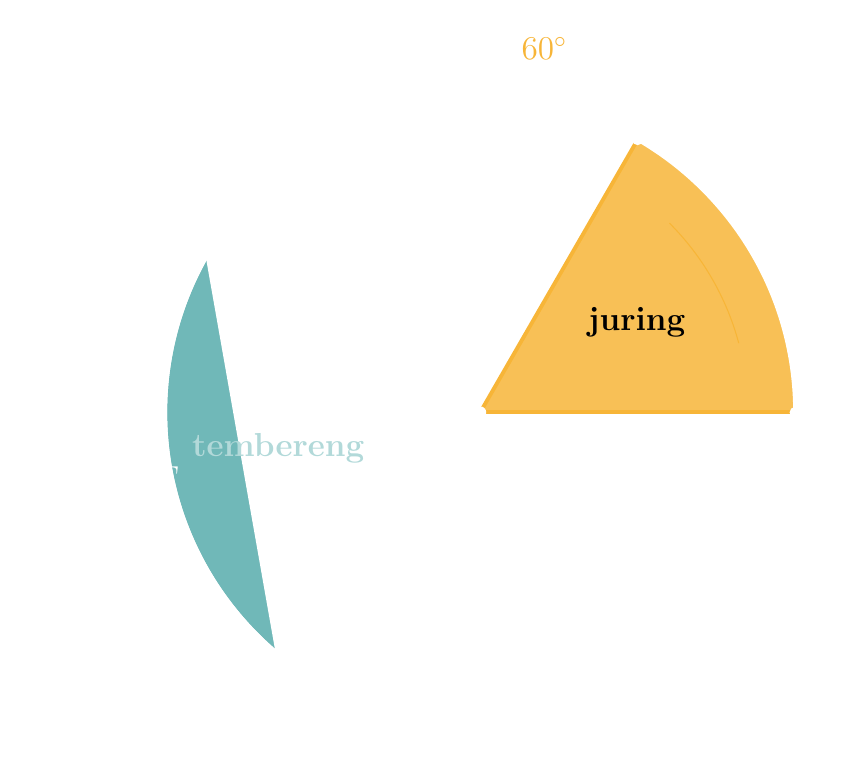
\begin{tikzpicture}[line width=1.4pt,text=white,font=\large]
  \coordinate (O) at (0,0);
  \coordinate (A) at (4,0);
  \coordinate (B) at (60:4);
  \coordinate (C) at (150:4);
  \coordinate (D) at (230:4);
  % Juring (kuning, dari 0 ke 60 derajat)
  \fill[acc,opacity=0.85] (O) -- (A) arc (0:60:4) -- cycle;
  \draw[acc] (O) -- (A);
  \draw[acc] (O) -- (B);
  % Tembereng (hijau muda, busur 150 ke 230)
  \coordinate (E) at (230:4);
  \fill[teal!70!white,opacity=0.8] (C) arc (150:230:4) -- cycle;
  \draw[white] (C) arc (150:230:4);
  \draw[white] (C) -- (E);
  % Lingkaran utama
  \draw[white] (O) circle (4);
  \draw[white] (O) -- (C);
  % Titik pusat dan label
  \fill[white] (O) circle (2.2pt);
  \node[below left=2pt] at (O) {$O$};
  % Label juring
  \node at (30:2.3) {\textcolor{black}{\textbf{juring}}};
  \node[acc] at (80:4.7) {$60^\circ$};
  \draw[acc,thin] (15:3.4) arc (15:45:3.4);
  % Label tembereng
  \node[teal!30!white] at (190:2.6) {\textbf{tembereng}};
  \node[white] at (190:4.8) {busur $EF$};
  % titik-titik
  \fill[white] (A) circle (2pt); \node[below right] at (A) {$A$};
  \fill[white] (B) circle (2pt); \node[above right] at (B) {$B$};
  \fill[white] (C) circle (2pt); \node[above left] at (C) {$E$};
  \fill[white] (E) circle (2pt); \node[below left] at (E) {$F$};
\end{tikzpicture}
\end{document}
